\subsection{High-Level System Design}
We first identify the complication of MPI code is on the message matching
mechanism. MPI point-to-point procedures (Send/Recv) facilitate matching
messages by tagging each with an integer in addition to destination and
communicator. The implementation uses several queues data structure to store
incoming requests and messages. For example, the unexpected queue store arrived
messages without a matching request; the posted queue will store the pending
requests without matching messages. Depending on different arrival order,
traversing, insertion or deletion of entries into queues will be issued. In a
concurrent setting, these are critical section that need to be protected. An
efficient lock-free control of these operations are non-existent even though
individual queue could be implemented efficiently.  Moreover, when the number
of concurrent communication increases, traversing a queue requires linear time
to the size of pending requests.

We propose an implementation MPI based on the following assumptions:
\begin{itemize}
  \item Large number of concurrent threads Threads are lightweight; they are
    scheduled by a user-space scheduler that understands synchronization
    objects.
  \item The implementation is optimized for the case where MPI_ANY_SOURCE and MPI_ANY_TAG are not used.
  \item No concurrent send and receive having the same signature, thus we do not yet worry about odering.
  \item The NIC can be accessed in user space; it has its own routing tables,
    in order to translate ranks in MPI\_COMM\_WORLD to physical node addresses;
    it has page tables, in order to translate virtual addresses to physical
    addresses.
  \item We consider only x86_64 machine, however the technique is general
    enough to port to other architecture which supports atomic exchange and
    atomic bit manimupation.
\end{itemize}

The key data structure for communication is a lock-free hash table which stores
both unsolicited incoming messages and outstanding receives. Since we assume
there are no wildcard, we can hash by source and tag. We focus on critical
operations, the creation of communicators or of datatypes is not (yet)
address. We also ignore, for the time being, one-sided operations.

The runtime is an integrated system of a user-level thread (ULT) scheduler and
a communication server. The ULT provides a low latency thread management while
the server is a kernel-thread dedicating to message delivery. The two
components interact using the afortmentioned hash-table.  Our primary goal is
to design an algorithm and optimize to minimize the latency of this
interaction. A failure to achieve this goal simply adds extranous overhead to
single threaded application and might not achieve significant benefit that
justifies its cost. We shall also show that our design allows optimization space
to be reduced to optimizing a few neccessary operations.

Resource management is another important issue. Aside from communication
context such as connections and NIC-provided control data which we maintains
per communication server, we have to maintain a pool of packets structure. The
pool is the second shared data structure of the runtime. The two basic operations
are \texttt{get} and \texttt{ret} which obtains and returns a packet from/to
the pool respectively. Each packet is used for storing control and message data
to deliver to network device.

\begin{figure*}[!ht]
  \centering
  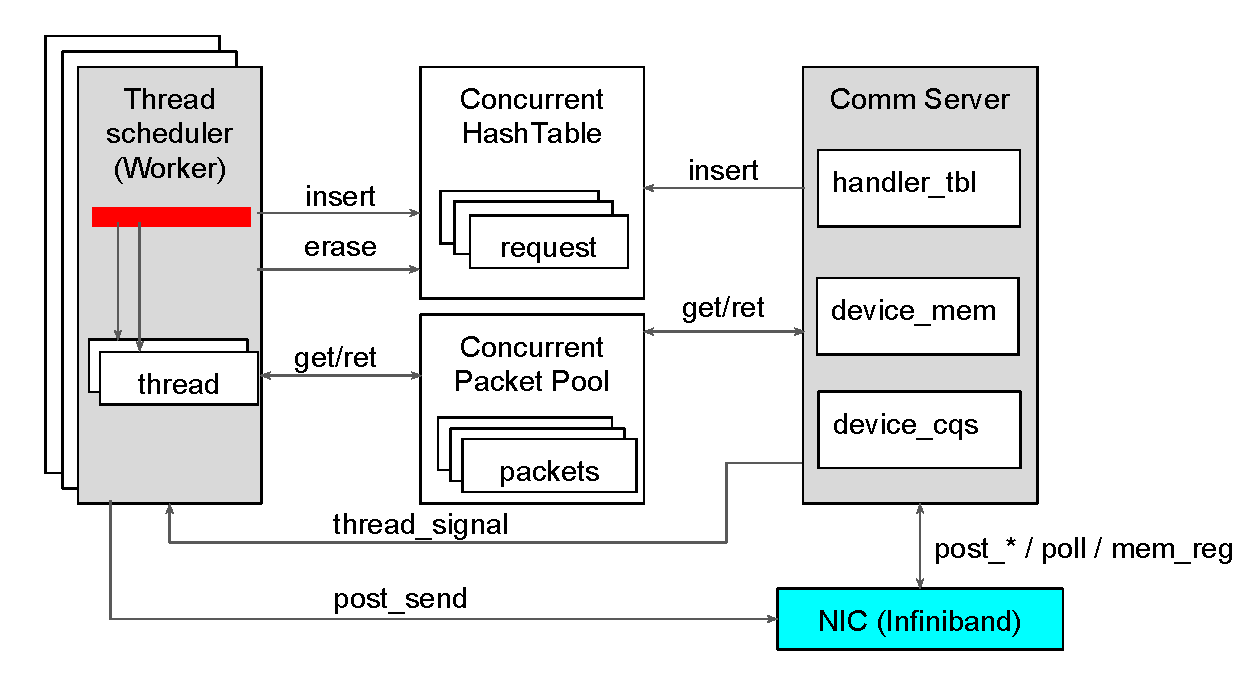
\includegraphics[width=.6\textwidth]{fig/runtime.pdf}
  \caption{MPI Runtime Architecture for multi-threaded executions}\label{fig:overall}
\end{figure*}

Figure \ref{fig:overall} shows the overall architecture of our described
runtime system.

\subsection{Point-to-Point Message Passing Algorithms}
We now describe an algorithm and its data structure that facilites the
point-to-point communication in Message Passing semantics. Our algorithm relies
on a specialized concurrent hash-table $H$ defined as follows.

We denote a tuple $(k,v) \in H$ when $v$ is stored in the hash-table using the
key $k$. At initialization, for any key $k$, only the tuple $(k,\bot)$ are
stored in the table. The hash-table has two operations: 

\begin{itemize}
  \item $H.\text{insert}(k,v)$: attempt to replace value of key $k$ by $v$.
  \item $H.\text{empty}(k)$: replace value of key $k$ by $\bot$
\end{itemize}

Additionally, let $H_t$ denote a state of $H$ which is a set of all key-value
pair stored in $H$ at time $t$, $H_{t_0}$ denote the state of $H$ before a
operation and $H_{t_1}$ denotes the state of $H$ after a operation;
$\mathbb{K}, \mathbb{V}$ denote the key and entry space. In a sequential
history, we have the following legal semantics:

\begin{equation}
  \text{insert}(k, v) = \left\{
    \begin{array}{@{}l@{\thinspace}l}
      v \iff (k,\bot) \in H_{t_0}, (k,v) \in H_{t_1}\\
      v' \iff (k,v') \in H_{t_0}, (k,v') \in H_{t_1}
    \end{array}
    \right.
\end{equation}
\begin{equation}
  \text{empty}(k) = \text{success} \iff  (k,v) \in H_{t_0}, (k,\bot) \in H_{t_1}
\end{equation}
\begin{equation}
  \forall k_0 \in \mathbb{K}, \nexists {(v_0, v_1) \in \mathbb{V}}
  \mid {{v_0 \ne v_1} \wedge \{(k_0, v_0), (k_0, v_1)\} \subset H_{t}}
\end{equation}

That is, (1) means that \texttt{insert} succeeds only if the entry being stored
with $k$ at the time of insertion is $\bot$.  In that case, $(k,\bot)$ is
replaced with $(k, v)$. Otherwise, the operations fail and existing value is
returned i.e. no changed are made to $H$. In contrast, \texttt{erase} as in (2)
is always successful, which replaces any value $v$ with the input $k$ with
$\bot$, essentially removing $v$ from the hash-table. The (3) equation is the
consistency requirement for hash-table, which means for each key we allow
only one value associated with it.

In a concurrent setting, we further require the hash-table to be
\textit{linearizable}.  This means we ensure firstly safety and correctness
property. Secondly, we ensure operations take affect in a real-time order.
This is a strong guarantee however is neccessary to implement MPI semantics
which have operations executed in program order. Lastly, linearizability is
\textit{composable} which allows us to correctly use the hash-table to
implement other concurrent objects.

Message delivery in general can be implemented in two way: \textit{eager} or \textit{rendevouz}
protocol. Eager protocol is used when the target buffer is not known to the
sender. Thus, an copy is made into an intermediate buffer - usually packed with
other control data to deliver to the network. This also allows the Send
operation to return immediately as the buffer can be reused.  This protocol
however becomes inefficient when message size gets larger, typically larger
than the L2 or L3 cache size i.e. the cost of data movement is significant.
When this is the case, we switch to rendevouz protocol in which the data is
delivered directly from the source buffer to the target buffer by the NIC thus
saving extra copies.  The protocol however requires some control messages to
exchange control data and signal completion.

\subsubsection{Eager protocol}

\begin{algorithm}
  \caption{Eager-message send/recv for thread}
  \label{algo:short}
  \begin{algorithmic}[1] % The number tells where the line numbering should start
    \Procedure{Send-Eager}{$b, s, d$} \Comment: buffer, size, destination signature 
      \State $p$ = pkpool.get()
      \State Set packet header $p.d$ to $d$
      \State Copy $b$ to $p.b$
      \State Post $p$ to network for send.
    \EndProcedure
    \\
    \Procedure{Recv-Eager}{$b, s, d$} \Comment: buffer, size, source signature 
      \State Create a request $r$ = $(b,s,d, (\omega, \Gamma))$
      \State Create hash-value $v$ from $r$.
      \State Create hash-key $k$ from $d$.
      \State $v' = H.\text{insert}(k,v)$
      \If {$v' \ne v$}
        \Comment: insertion fail
        \State Copy $v'.p.b$ to $b$
        \Comment: message arrived, copy data.
        \State pkpool.ret($p$)
      \Else
        \Comment: insertion success
        \State \texttt{ThreadWait}()
        \Comment: message not arrived, wait.
      \EndIf
      \State $H.\text{erase}(k)$
    \EndProcedure
  \end{algorithmic}
\end{algorithm}

\begin{algorithm}
  \caption{Eager-message packet handler for communication server}
  \label{algo:server-short}
  \begin{algorithmic}[1]
    \Procedure{Recv-Eager-Packet}{p}
      \State Create hash-value $v$ from $p$.
      \State Create hash-key $k$ from $p.d$.
      \State $v' = H.\text{insert}(k,v)$
      \If {$v' \ne v$}
        \Comment: insertion fail.
        \State Copy $p.b$ to $v'.r.b$
        \Comment: thread arrived, copy data.
        \State \texttt{ThreadSignal}($r.\Gamma$)
        \State pkpool.ret($p$)
      \Else
        \Comment: insertion success.
        \State \Return
        \Comment: thread not arrive, nothing to do.
      \EndIf
    \EndProcedure
  \end{algorithmic}
\end{algorithm}

The pseudocode for eager protocol is listed in Algorithm \ref{algo:short} and
\ref{algo:server-short} for worker thread and communication server
respectively. There is not much for the eager send, the thread can return
immediately without any waiting since the content of the data shall be copied
over to the packet data for transfering. Only the receiving algorithm needs some
elaborations. The basic idea here is that the thread and the communication
server could use the results from hash-table insertion to coordinate the
matching of messages and request.

The hashing function takes the request signature (rank, tag, communicator) and
produces a 64-bit key for inserting into the table. It is easy to see that
when there is a matching message and request, both the server and a thread 
are having the same signature and key. Depending on which comes first the algorithm
goes into two cases. If the communication server succeeds with the hash
insertion, the server knows the receiving request has not been posted and it
returns immediately. A thread later comes, eventually fails the insertion but
finds a packet with the needed data to work with. On the other hand, if the
thread is the one who succeeds, the request is then inserted into the
hash-table with the synchronization object.  The thread is yielded by executing
\texttt{ThreadWait}. The worker is now free to do other works. When the
associated packet arrived, the server will fail the insertion and find the
request with the attached synchronization object. It now can mark the thread as
schedulable using \texttt{ThreadSignal} so when the worker is available it will
pick up the works with the available data.

Since there is no need for linear searching, our matching algorithm achieves a
constant time complexity as long as operation of thread scheduler, pool and
hash-table is also constant time.

\subsubsection{Rendevouz protocol}
A rendevouz protocol have the same algorithm as short protocol after we have
exchanged the control message via eager-protocol. The control messages 
includes two messages: a RTS (ready-to-send) issued by the sender, a RTR
(ready-to-receive) issued by the receiver. By then, the sender and the receiver
has known the addresses of each other buffer and they can perform
communication.  The data transfer could be optimized further using the
Remote Direct Memory Access (RDMA) feature of modern Network Interface
Controller (NIC).  Several researchs has focused on optimizing this operation.

As an effect of our assumption, in this protocol we can save one control
message i.e. the RTS.  The reason is we do not have wild-card, the sender and
receiver knows exactly their target.  We only require the receiver to send its
buffer to the sender. The sender can follow up by issuing an RDMA.  Analogous
to the eager protocol, whenever the sender or receiver is required to wait for
a matching message it will perform \texttt{ThreadWait}, and later when the
message has arrived the communication server will perform a
\texttt{ThreadSignal}.

Specifically, the sender waits when the RTR message has not arrived or when
RDMA is pending. In both situation the server wake up the sender thread when
RDMA has completed. The receiver after issuing the RTR will wait until the
signal that RDMA has finished arrived and data is now available.

\subsection{Critical Operations Discussion}
Clearly, optimizing the hash-table, the packet pool and the thread scheduler
operations are the key to achieve good performance for our protocols. One could
achieve $O(1)$ amortized in complexity however, an efficient implementation
requires optimizing for the constant factor. Ideally, we want these operations
to be \textit{wait-free} (every operation has a bound on number of steps before
completion) to ensure progress and guarantee system-wide throughput. Moreover, we 
want to minimize memory accesses thus reducing possible cache miss. In the next
section, we describe the implementaion of each of the three components and show
how we could optimize toward our goals.

\subsection{Supporting wild-cards}
Although it is out of the scope of this paper to deal with wild-cards, we
provide here some possible options to mitigate existing applications. A
MPI-complete implementation could be built on top of our foundation but
possibly losing some of the properties that we want for performance. However,
among the applications that we have looked at, these mitigation approaches are
often sufficient.

An application depending on \texttt{MPI_ANY_TAG} can be rewritten such
that the receiver can have a tag (Note that the sender always has a valid tag).
There are two cases:
\begin{itemize}
  \item Number of expecting tags are bounded and deterministic: one can spawn a
    number of threads, each posts a \texttt{MPI_Recv} for a valid expecting
    tag and subsequently performs actions associating with that tag. 
  \item The number of tags is un-bounded or non-deterministic: the sender
    can help by first sending its tag to the receiver via a pre-defined tag.
    Once sender and receiver agrees on the generated tag, they can proceed
    the communication.
\end{itemize}

The remedy for \texttt{MPI_ANY_SOURCE} is similar to \texttt{MPI_ANY_TAG} when
there is a bounded and deterministic number of source ranks. It is harder in
the other case since there is no way to notify the receiver of its sender
unless there is a 3rd-party channel. For example, we could introduce a special
\texttt{MPI_Send_anysource} procedure, in which the sender expects the receiver
to post a \texttt{MPI_ANY_SOURCE}. In that case, when the sender receives this
special packet, it will ignore the rank of the sender and uses a special tag
associated with \texttt{MPI_ANY_TAG} to match into the hash-table.

When there is concurrent send/recv with the same signature (rank, tag,
communicator), one can add to the tag value a session counter increasing
atomically with each send/recv posted message to ensure order. When this is not
possible, relaxing the hash-table to allow redundant entries with the same key
is required. We refer the reader to an alternative algorithm introduced
recently by Intel to allow matching using such hash-tables \cite{m5}. 
